%%This is a very basic article template.
%%There is just one section and two subsections.
\documentclass[12pt, twoside]{article}

\usepackage[francais]{babel}
\usepackage[T1]{fontenc}
\usepackage[latin1]{inputenc}
\usepackage[left=2cm, right=2cm, top=6mm, bottom=1cm]{geometry}
\usepackage{float}
\usepackage{graphicx}
\usepackage{array}
\usepackage{multirow}
 
\begin{document}

\section*{\center{Devoir maison 1 }}

\enskip Devoir � rendre pour le samedi 20 septembre 2008.

\begin{tabular}{cc}
\begin{minipage}{11cm}
\textbf{Exercice 1:}
On consid�re un carr� $ABCD$ de c�t� $1$. Le point $I$ est le milieu de $[AB]$.
Le cercle de centre $I$ de rayon $IC$ coupe la demi-droite $[IB)$ en $P$.\\
1) Calculer les distances $IB$, $IC$ puis $AP$.\\
2) On note $\Phi=\frac{1+\sqrt{5}}{2}$ ($\Phi$ se lit ``phi'' et s'appelle le
nombre d'or). Montrer que $AP*BP=AB^{2}$, en d�duire$\frac{AP}{AB}=\frac{AB}{BP}=\Phi$. 
(\textit{indication}: penser � �crire $AP*BP=AB*AB$)
\end{minipage}
&
\begin{minipage}{6cm}
\begin{center}
	  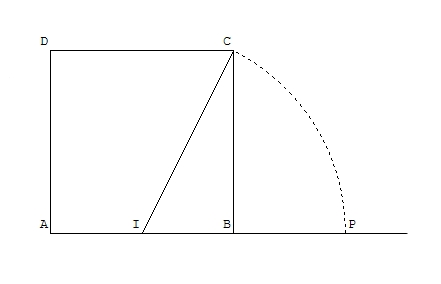
\includegraphics[width=8cm]{images/exo3.jpg}
\end{center}
\end{minipage}
\end{tabular}

\enskip \textit{Remarque}: la suite de l'exercice peut se faire sans cette
question.

\medskip
 \enskip A votre avis, quelle est la nature de $\Phi$? (on ne demande pas la
justification). 


\enskip 3) Calculer $\Phi^{2}$ et montrer que $\Phi^{2}=\Phi +1$.

\bigskip
\bigskip

\begin{tabular}{cc}
\begin{minipage}{11cm}
\textbf{Exercice 2:}
Soient $[OB)$ et $[OC)$ deux demi-droites d'origine $O$. Les droites $(AI)$
et $(BC)$ sont parall�les. Le nombre au dessous d'une lettre majuscule est son
abscisse. On suppose les graduations de $[OB)$ r�guli�res.

\bigskip
Quel est le nombre $x$ ainsi construit? Justifier. Donner la nature de $x$.
(\textit{indication}: de la r�gularit� des graduations, on peut d�duire l'abscisse de $B$)
\end{minipage}
&
\begin{minipage}{6cm}
    \begin{center}
  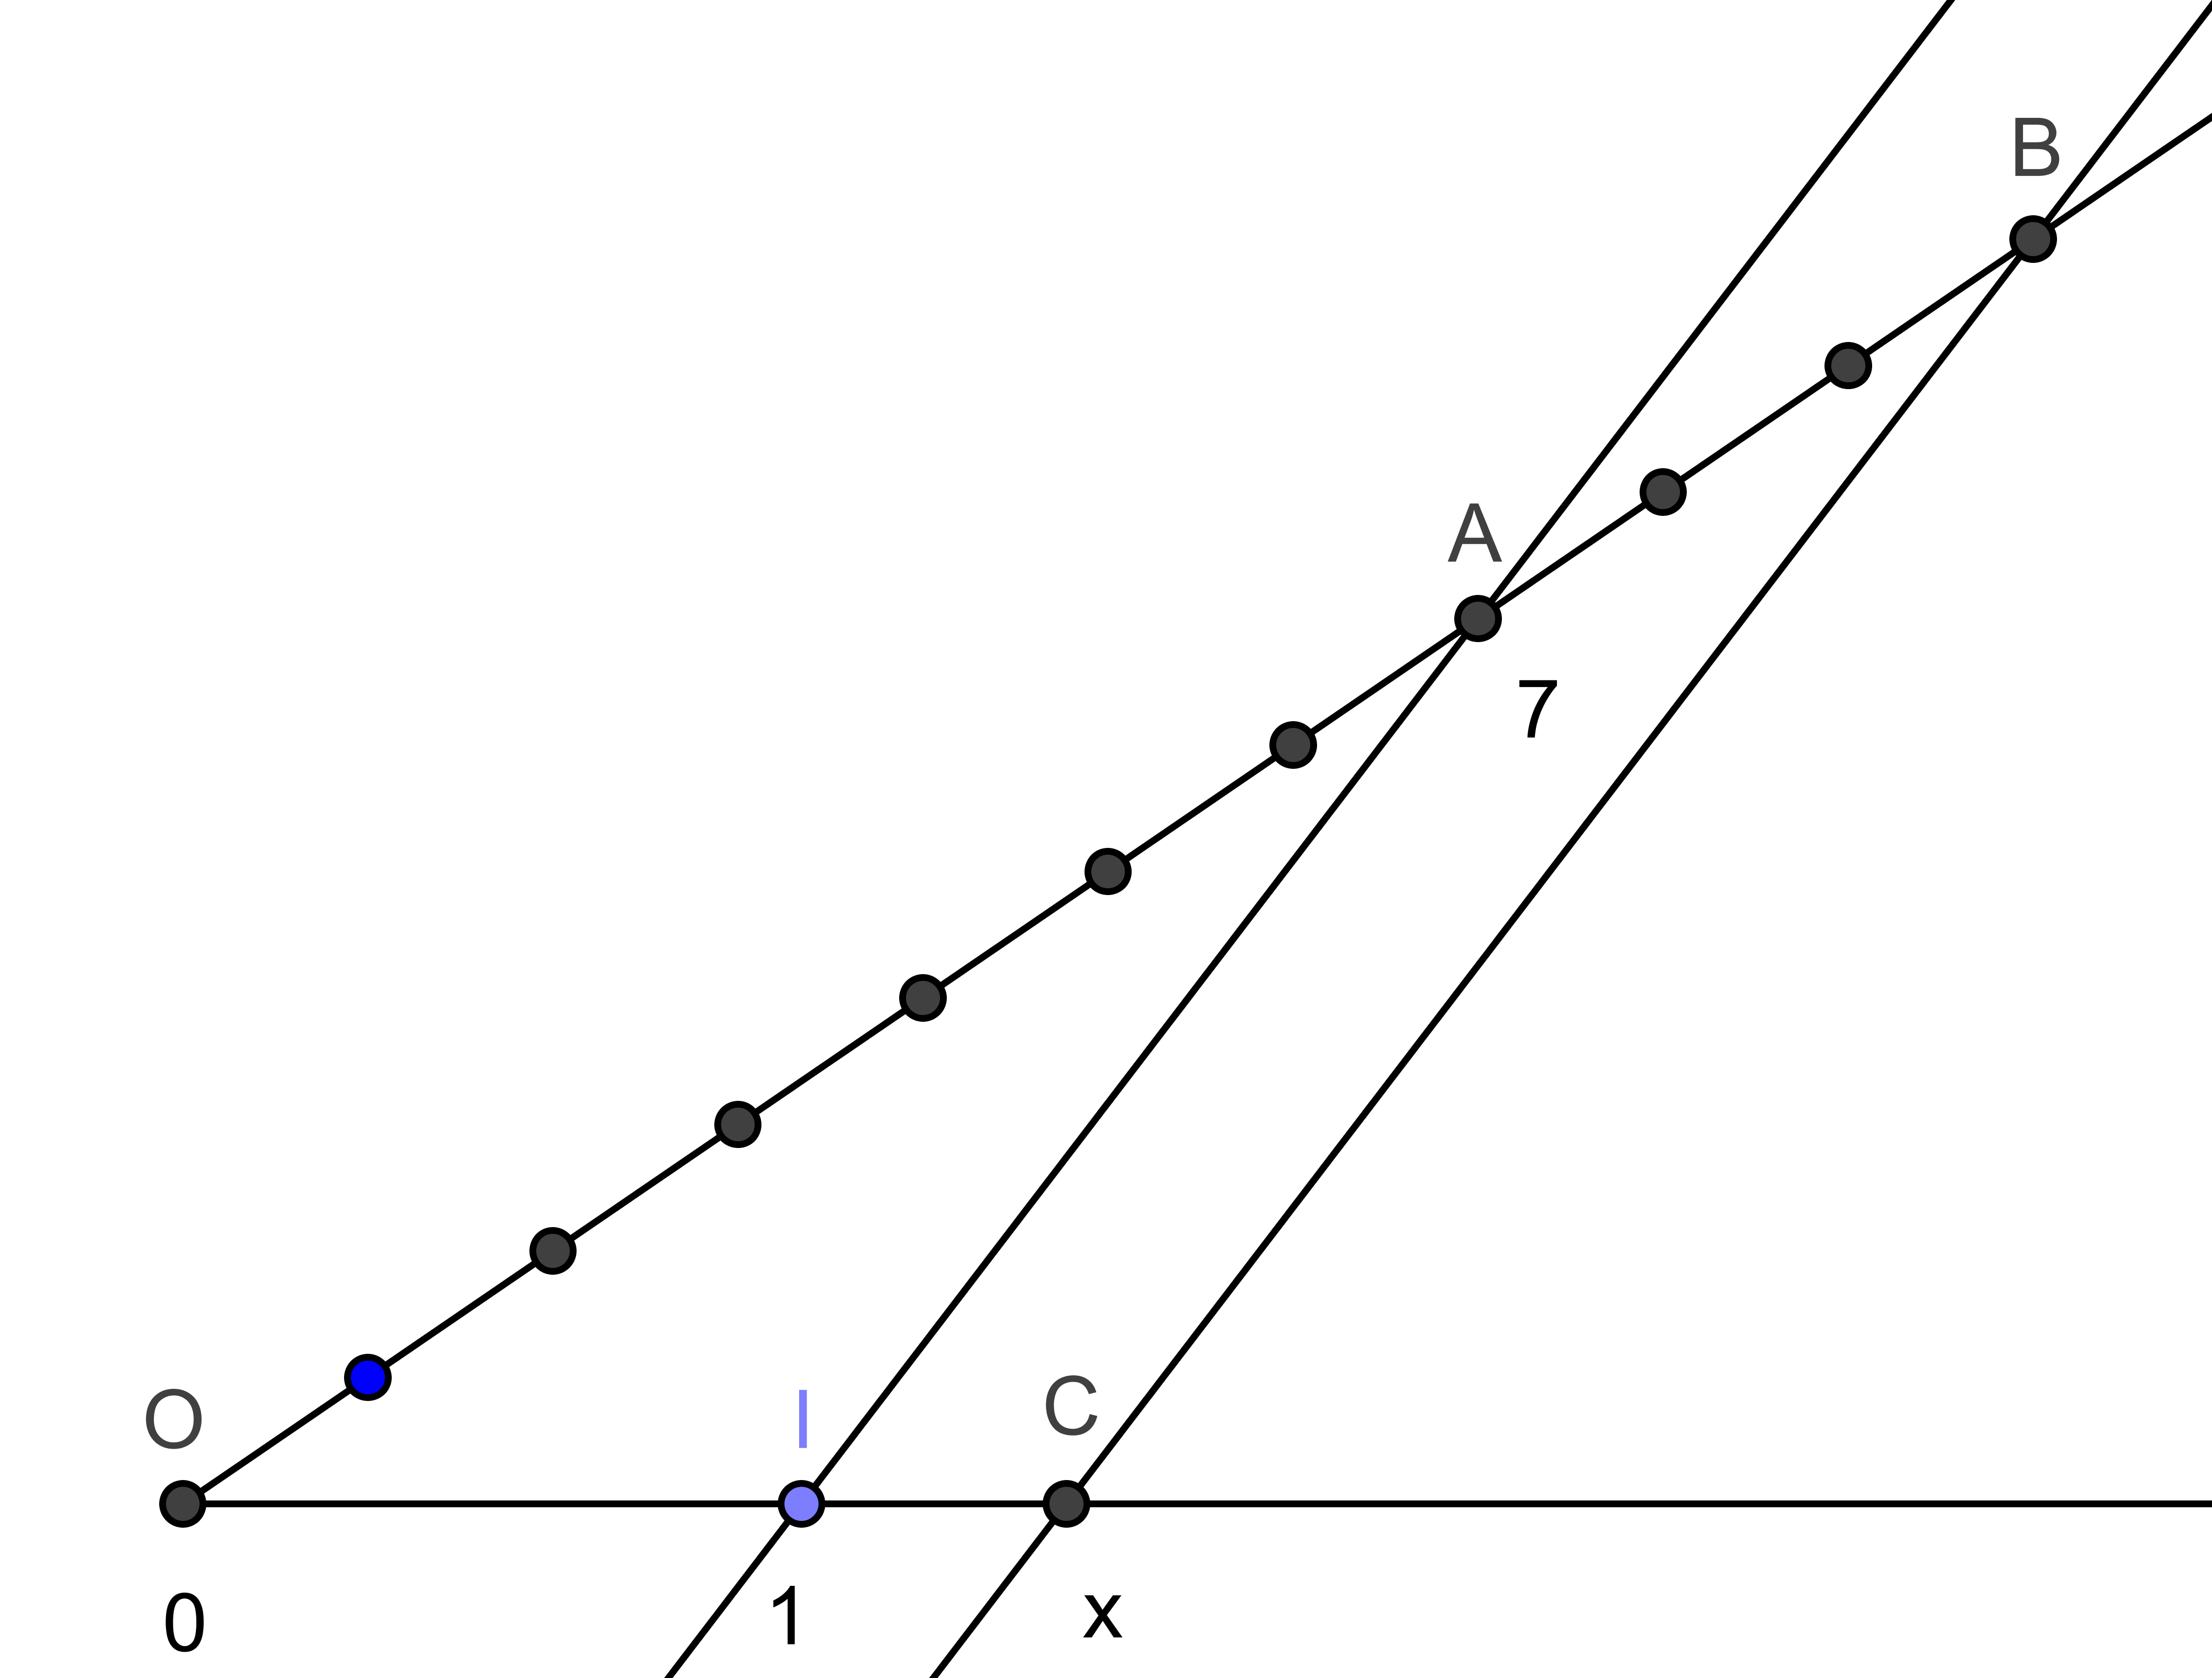
\includegraphics[width=6cm]{images/thales.png}
    \end{center}
 \end{minipage}
\end{tabular}

\bigskip
\bigskip


\textbf{Exercice 3:}
En utilisant la d�composition en facteurs premiers,calculer les expressions
suivantes: 


(d�tailler vos calculs)
\begin{enumerate}
  \item \large{$\frac{3*\sqrt{297}*\sqrt{616}*2}{\sqrt{396}^{2}}$}
  \item \large{$\frac{2}{77}-\frac{1}{28}+\frac{5}{22}$}
  \item \normalsize{le $pgcd$ de $207$ et de $132$}
  \item \large{$\frac{234*75}{90*28}$} \normalsize{(sous forme de fraction
  irr�ductible)}
\end{enumerate}

\bigskip
\bigskip

\textbf{Exercice 4:} Soit $x$ le nombre $0,999999 \ldots$ , justifier que
$10x=9+x$. En d�duire la valeur de $x$.


Quelle est la nature de $x$?


\textit{Rappel:} $0,999999 \dots$  signifie qu'il y a une infinit� de $9$ apr�s
la virgule.

\bigskip
\bigskip
\textbf{Exercice 5: A la mani�re de Fermat}

\begin{enumerate}
  \item On souhaite d�composer le nombre $667$. 
\begin{enumerate}
  \item  Ce nombre est il divisible par l'un des nombres premiers inf�rieurs �
  $15$? Pour le d�composer, nous allons � la mani�re de Fermat, transformer son
  �criture.
  \item V�rifier que $667= 26^{2}-9$.
  \item En d�duire la d�composition en facteurs premiers de $667$.
\end{enumerate}
  \item A l'aide de votre calculatrice, transformer de m�me l'�criture du
  nombre $437$ pour trouver sa d�composition en produit de facteurs premiers. 
\end{enumerate}

\end{document}
